\begin{latin}
	\hspace*{-0.04\linewidth}
	\footnotesize
	\begin{subfigure}[t]{0.45\textwidth}
	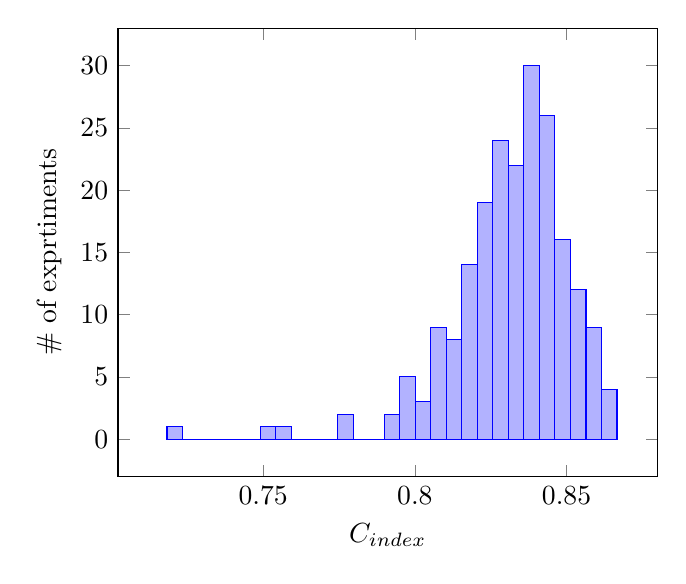
\begin{tikzpicture}
	\begin{axis}[
	area style,
	xtick={0.70, 0.75, ..., 0.85},
	ytick={0, 5, ..., 40},
	xmax=0.88,
	ylabel=\# of exprtiments,
	xlabel=$C_{index}$
	]
	\addplot+[ybar interval,mark=no] plot coordinates {
		(0.7183191, 1.0)
		(0.723433, 0.0)
		(0.7285468, 0.0)
		(0.7336607, 0.0)
		(0.7387746, 0.0)
		(0.7438885, 0.0)
		(0.7490023, 1.0)
		(0.7541162, 1.0)
		(0.7592301, 0.0)
		(0.764344, 0.0)
		(0.7694578, 0.0)
		(0.7745717, 2.0)
		(0.7796856, 0.0)
		(0.7847995, 0.0)
		(0.7899134, 2.0)
		(0.7950272, 5.0)
		(0.8001411, 3.0)
		(0.805255, 9.0)
		(0.8103689, 8.0)
		(0.8154827, 14.0)
		(0.8205966, 19.0)
		(0.8257105, 24.0)
		(0.8308244, 22.0)
		(0.8359382, 30.0)
		(0.8410521, 26.0)
		(0.846166, 16.0)
		(0.8512799, 12.0)
		(0.8563937, 9.0)
		(0.8615076, 4.0)
		(0.8666215, 2.0)
	};
	\end{axis}
	\end{tikzpicture}
	\caption{Exhaustive Search}
	\end{subfigure}
	\hfill
	\begin{subfigure}[t]{0.45\textwidth}
	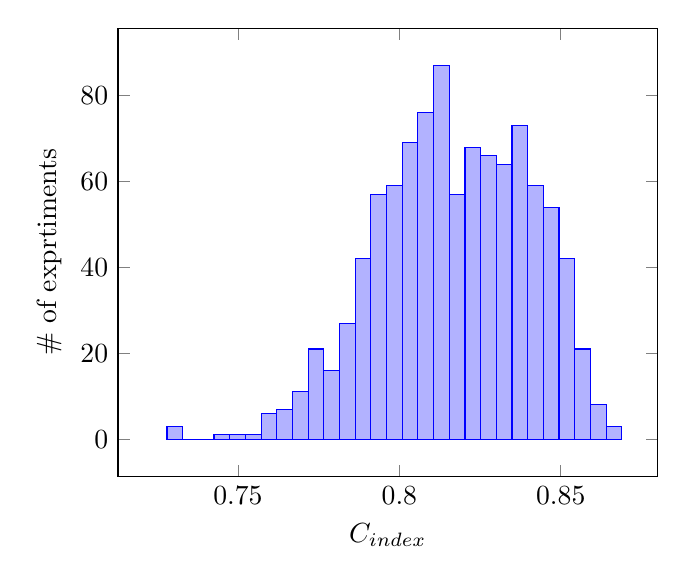
\begin{tikzpicture}
	\begin{axis}[
	area style,
	xtick={0.70, 0.75, ..., 0.85},
	ytick={0, 20, ..., 160},
	xmax=0.88,
	ylabel=\# of exprtiments,
	xlabel=$C_{index}$
	]
	\addplot+[ybar interval,mark=no] plot coordinates {
		(0.7280231, 3.0)
		(0.7328811, 0.0)
		(0.737739, 0.0)
		(0.742597, 1.0)
		(0.747455, 1.0)
		(0.752313, 1.0)
		(0.757171, 6.0)
		(0.762029, 7.0)
		(0.7668869, 11.0)
		(0.7717449, 21.0)
		(0.7766029, 16.0)
		(0.7814609, 27.0)
		(0.7863189, 42.0)
		(0.7911768, 57.0)
		(0.7960348, 59.0)
		(0.8008928, 69.0)
		(0.8057508, 76.0)
		(0.8106088, 87.0)
		(0.8154668, 57.0)
		(0.8203247, 68.0)
		(0.8251827, 66.0)
		(0.8300407, 64.0)
		(0.8348987, 73.0)
		(0.8397567, 59.0)
		(0.8446147, 54.0)
		(0.8494726, 42.0)
		(0.8543306, 21.0)
		(0.8591886, 8.0)
		(0.8640466, 3.0)
		(0.8689046, 1.0)
	};
	\end{axis}
	\end{tikzpicture}
	\caption{Semi-Exhaustive Search}
	\end{subfigure}
\end{latin}